\documentclass[reprint, english, nofootinbib]{revtex4-2}

\usepackage{graphicx}
\usepackage{subfig}
\usepackage[colorlinks=true,urlcolor=blue,citecolor=blue]{hyperref}
\usepackage{physics}
\usepackage{amsmath}
\usepackage{amssymb}
\usepackage{amsbsy}
%\usepackage{bbold}
\usepackage{subfig}

\usepackage{blindtext}
\usepackage{tikzducks}
\usepackage{listings}

\graphicspath{{../figs/}}

\begin{document}
\title{Classification and Regression\\
\normalsize{From Linear and Logistic Regression to Neural Networks}}

\author{Nicholas Karlsen}
\affiliation{University of Oslo}
\author{Thore Espedal Moe}
\affiliation{University of Oslo}
\date{\today}

\begin{abstract}
\end{abstract}

\maketitle

\section{Introduction}

\section{Theory}
\subsection{Stochastic Gradient Descent}
\noindent
Consider a cost function in the form
\begin{equation}
    C(\pmb Y, \tilde{\pmb Y}(\pmb w)) = \frac{1}{N}\sum_{i=1}^{N}C_i(\pmb y_i, \tilde{\pmb y}(\pmb w)_i)
\end{equation}
for a data set $\pmb Y = \left\{\pmb y_1, \dots, \pmb y_N\right\}$ and a corresponding set of modeled data points $\tilde{\pmb Y}(\pmb w) = \left\{\tilde{\pmb y_1}(\pmb w), \dots, \tilde{\pmb y}_N(\pmb w)\right\}$, where the $C$ is some measure of the error of the model.

Given that our model is optimized by some set of weights $\pmb w$, we may optimize it by gradient descent, where the set of weights $\pmb w$ are updated by
\begin{equation}
    \pmb w^{(k+1)} = \pmb w^{(k)} - \eta \nabla_{w}C(\pmb Y, \tilde{\pmb Y})
\end{equation}
untill the cost function has reached a minima. However, we may not guarantee that this minima is infact the global minima of the cost function.

\begin{figure}[h!tb]
    \center
    \vspace{5mm} % To avoid touching the preceding text
    


\tikzset{every picture/.style={line width=0.75pt}} %set default line width to 0.75pt

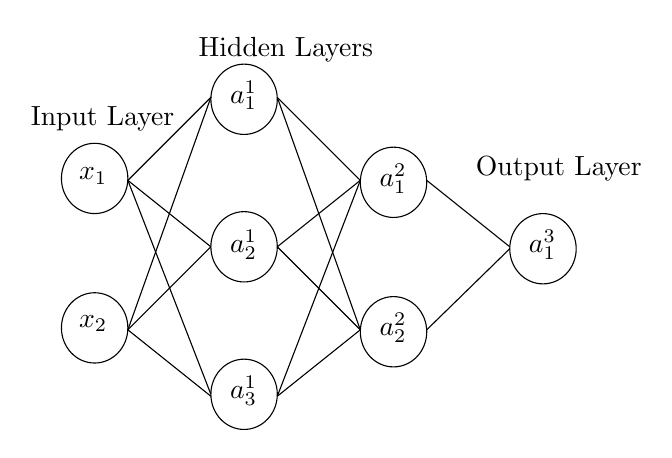
\begin{tikzpicture}[x=0.6pt,y=0.6pt,yscale=-1,xscale=1]
%uncomment if require: \path (0,484); %set diagram left start at 0, and has height of 484

%Flowchart: Connector [id:dp6019250960891445]
\draw  [fill={rgb, 255:red, 255; green, 255; blue, 255 }  ,fill opacity=1 ] (40,112.83) .. controls (40,101.14) and (48.95,91.67) .. (60,91.67) .. controls (71.05,91.67) and (80,101.14) .. (80,112.83) .. controls (80,124.52) and (71.05,134) .. (60,134) .. controls (48.95,134) and (40,124.52) .. (40,112.83) -- cycle ;
%Flowchart: Connector [id:dp8334547170271857]
\draw  [fill={rgb, 255:red, 255; green, 255; blue, 255 }  ,fill opacity=1 ] (40,202.83) .. controls (40,191.14) and (48.95,181.67) .. (60,181.67) .. controls (71.05,181.67) and (80,191.14) .. (80,202.83) .. controls (80,214.52) and (71.05,224) .. (60,224) .. controls (48.95,224) and (40,214.52) .. (40,202.83) -- cycle ;
%Flowchart: Connector [id:dp7153685420206096]
\draw  [fill={rgb, 255:red, 255; green, 255; blue, 255 }  ,fill opacity=1 ] (130,65.17) .. controls (130,53.48) and (138.95,44) .. (150,44) .. controls (161.05,44) and (170,53.48) .. (170,65.17) .. controls (170,76.86) and (161.05,86.33) .. (150,86.33) .. controls (138.95,86.33) and (130,76.86) .. (130,65.17) -- cycle ;
%Flowchart: Connector [id:dp5622283646258179]
\draw  [fill={rgb, 255:red, 255; green, 255; blue, 255 }  ,fill opacity=1 ] (130,154) .. controls (130,142.31) and (138.95,132.83) .. (150,132.83) .. controls (161.05,132.83) and (170,142.31) .. (170,154) .. controls (170,165.69) and (161.05,175.17) .. (150,175.17) .. controls (138.95,175.17) and (130,165.69) .. (130,154) -- cycle ;
%Flowchart: Connector [id:dp16862921724788715]
\draw  [fill={rgb, 255:red, 255; green, 255; blue, 255 }  ,fill opacity=1 ] (130,242.83) .. controls (130,231.14) and (138.95,221.67) .. (150,221.67) .. controls (161.05,221.67) and (170,231.14) .. (170,242.83) .. controls (170,254.52) and (161.05,264) .. (150,264) .. controls (138.95,264) and (130,254.52) .. (130,242.83) -- cycle ;
%Flowchart: Connector [id:dp4149695521858179]
\draw  [fill={rgb, 255:red, 255; green, 255; blue, 255 }  ,fill opacity=1 ] (220,115.17) .. controls (220,103.48) and (228.95,94) .. (240,94) .. controls (251.05,94) and (260,103.48) .. (260,115.17) .. controls (260,126.86) and (251.05,136.33) .. (240,136.33) .. controls (228.95,136.33) and (220,126.86) .. (220,115.17) -- cycle ;
%Flowchart: Connector [id:dp840876892841651]
\draw  [fill={rgb, 255:red, 255; green, 255; blue, 255 }  ,fill opacity=1 ] (220,205.17) .. controls (220,193.48) and (228.95,184) .. (240,184) .. controls (251.05,184) and (260,193.48) .. (260,205.17) .. controls (260,216.86) and (251.05,226.33) .. (240,226.33) .. controls (228.95,226.33) and (220,216.86) .. (220,205.17) -- cycle ;
%Flowchart: Connector [id:dp10784935111712701]
\draw  [fill={rgb, 255:red, 255; green, 255; blue, 255 }  ,fill opacity=1 ] (310,155.17) .. controls (310,143.48) and (318.95,134) .. (330,134) .. controls (341.05,134) and (350,143.48) .. (350,155.17) .. controls (350,166.86) and (341.05,176.33) .. (330,176.33) .. controls (318.95,176.33) and (310,166.86) .. (310,155.17) -- cycle ;
%Straight Lines [id:da7667435970573455]
\draw    (80,114) -- (130,154) ;
%Straight Lines [id:da48448129133283535]
\draw    (170,154) -- (220,114) ;
%Straight Lines [id:da4471635916327932]
\draw    (260,114) -- (310,154) ;
%Straight Lines [id:da5105417767244789]
\draw    (80,204) -- (130,244) ;
%Straight Lines [id:da6281305874976782]
\draw    (170,154) -- (220,204) ;
%Straight Lines [id:da9404110386397875]
\draw    (260,204) -- (310,155.17) ;
%Straight Lines [id:da669909761533326]
\draw    (130,154) -- (80,204) ;
%Straight Lines [id:da03861624272354913]
\draw    (80,204) -- (130,64) ;
%Straight Lines [id:da7865539839743194]
\draw    (80,114) -- (130,64) ;
%Straight Lines [id:da006395151871996019]
\draw    (170,64) -- (220,114) ;
%Straight Lines [id:da6703248416054105]
\draw    (170,64) -- (220,204) ;
%Straight Lines [id:da568582824840071]
\draw    (170,244) -- (220,204) ;
%Straight Lines [id:da5603512527475397]
\draw    (170,244) -- (220,114) ;
%Straight Lines [id:da15589575659778376]
\draw    (80,114) -- (130,242.83) ;

% Text Node
\draw (49,105) node [anchor=north west][inner sep=0.75pt]    {$x_{1}$};
% Text Node
\draw (49,194) node [anchor=north west][inner sep=0.75pt]    {$x_{2}$};
% Text Node
\draw (140,52.33) node [anchor=north west][inner sep=0.75pt]    {$a^{1}_{1}$};
% Text Node
\draw (140,142.33) node [anchor=north west][inner sep=0.75pt]    {$a^{1}_{2}$};
% Text Node
\draw (140,230) node [anchor=north west][inner sep=0.75pt]    {$a^{1}_{3}$};
% Text Node
\draw (230,102.33) node [anchor=north west][inner sep=0.75pt]    {$a^{2}_{1}$};
% Text Node
\draw (230,192.33) node [anchor=north west][inner sep=0.75pt]    {$a^{2}_{2}$};
% Text Node
\draw (320,142.33) node [anchor=north west][inner sep=0.75pt]    {$a^{3}_{1}$};
% Text Node
\draw (20,68) node [anchor=north west][inner sep=0.75pt]   [align=left] {Input Layer};
% Text Node
\draw (288,98) node [anchor=north west][inner sep=0.75pt]   [align=left] {Output Layer};
% Text Node
\draw (185,35) node   [align=left] {\begin{minipage}[lt]{74.80000000000001pt}\setlength\topsep{0pt}
Hidden Layers
\end{minipage}};


\end{tikzpicture}

    \caption{\label{fig: NN Fig} Visual representation of a simple neural network with $2$ inputs, $2$ hidden layers with $3$, $2$ neurons respectively and an output layer with a single neuron.}
\end{figure}

\subsection{Feed-Forward Neural Network}
\noindent
We initialize the Feed-Forward algorithm by computing
\begin{align}\label{eqn: FeedForward Initial}
    \begin{split}
        z^1_j &= w^1_{jk}X_k + b^1_j \\
        a^1_j &= \sigma(z^1_j)
    \end{split}
\end{align}
where we adopt the Einstein summation convention by summing over repeated indices.
We then compute
\begin{align}
    \begin{split}
        z^l_{j} &= w^l_{jk}a^{l-1}_k + b^l_j \\
        a^l_{j} &= \sigma(z^l_{j})
    \end{split}
\end{align}
for hidden layers $l = 2, \dots, L$. Then, for the ouput layer we compute
\begin{align}
    \begin{split}
        z^{L}_j &= w^{L}_{jk}a^{L-1}_k + b^{L}_j \\
        a^{L}_j &= \tilde\sigma(z^{L}_j)
    \end{split}
\end{align}
where $a^{L}_j$ is the predicted response, and $\tilde\sigma$ is the activation function for the output layer, which may differ from the activation function of the hidden layers.

We then compute the error of the output as
\begin{equation}
    \delta^{L}_j = \pdv{C}{a^{L}_{j}} \odot \tilde\sigma'(z^{L}_j)
\end{equation}
and backpropogate the error like
\begin{equation}
    \delta^{l}_j = \qty(\delta^{l+1}_{k}\qty(w^{l+1}_{kj})^T) \odot \sigma'(z^l_j)
\end{equation}
for all $l = L-1, \dots, 2$.

We may then easily compute the gradients of the cost function wrt. the weights \& biases as

\begin{align}
    \begin{split}
        \pdv{C}{w_{jk}^l} &= \delta_j^l a^{l-1}_k \\
        \pdv{C}{b^l_j} &= \delta_j^l
    \end{split}
\end{align}
which are then used to update the weights and biases via gradient descent.

\section*{Backpropogation with minibatches}
We have input and output matrices $X\in[M\times P], Y\in[M\times Q]$, with elements $X_{mp}, Y_{mq}$. Since we wish to perform the Backpropogation effectively using the highly optimized linear algebra libraries available in Numpy, we must therefore slightly alter the way in which we perform the backpropogation. Since our input vectors $X$ now comes in the form

\begin{equation}
    X = \qty[
    \begin{matrix}
        X_1 \\ \vdots \\ X_P
    \end{matrix}
    ] \rightarrow
    X = \qty[
    \begin{matrix}
        X_{11} & \dots & X_{1P} \\
                 & \vdots&          \\
        X_{M1} & \dots & X_{MP}
    \end{matrix}
    ]
\end{equation}
we let $z^l_j \rightarrow z^l_{mj}$ and $a^l_{j}\rightarrow a^l_{mj}$ such that they are in accordance with $X_{mp}, Y_{mq}$.

In order to adhere to this new form, we must transpose Eqn.~\ref{eqn: FeedForward Initial} which yields
\begin{equation}
    w_{jk}X_K \rightarrow \qty(w_{jk}X_k)^T = X_k^T \qty(w^1_{kj})^T
\end{equation}
Thus, we may write the initial step as
\begin{align}
    \begin{split}
        z^1_{mj} &= X_{mk}w_{kj} + \qty(b^1_j)^T \\
        a^1_{mj} &= \sigma\qty(z^1_{mj})
    \end{split}
\end{align}
where the transposed bias is implicitly added element-wise to each row in the resultant matrix. In a similar fashion, we feed forward for $l = 2, \dots L$
\begin{align}
    \begin{split}
        z^l_{mj} &= a^{l-1}_{mk}w_{kj} + \qty(b^L_j)^T \\
        a^l_{mj} &= \sigma(z^L_{mj})
    \end{split}
\end{align}
and for the output layer
\begin{align}
    \begin{split}
        z^L_{mj} &= a^{L-1}_{mk}w_{kj} + \qty(b^L_j)^T \\
        a^L_{mj} &= \tilde\sigma\qty(z^L_{mj})
    \end{split}
\end{align}

\begin{equation}
    \delta^{l}_j = (w_{jk})^T \delta^{l+1}_j
\end{equation}
\begin{equation}
    \delta^{l}_{mj} = \delta^{l+1}_{mk}w^{l+1}_{kj}
\end{equation}


\section{Results \& Discussion}
\section{Conclusion}

\onecolumngrid
\bibliography{bibfile}
\newpage
\twocolumngrid
\appendix
\end{document}
